\section{Completed Evidence, Resource Audits, and Controlled Follow-ups}\label{app:evidence-extension}
All comparisons below use seed 42. A two-rate result requires both rates for every method, and all prescribed epochs must finish. Rates and exploratory flag-step settings are selected on validation only. Incomplete configurations remain in the execution counts, without extrapolated endpoints.
\paragraph{Proposal coverage and remaining work.} Configuration counts measure execution coverage, not positive results. The graph and tabular grids are complete; image and continual-learning runs continue; the LSTM grid has nine completed candidates and one recorded failure. WikiText-2 epochs traverse its full corpus; GPT-2 uses fixed ten-step evaluation units, explicitly not corpus epochs or the 1000-corpus-epoch-equivalent proposal budget. OpenWebText/C4 subsets and corpus-switch experiments are not established completed benchmarks in this matrix. Core50 and DomainNet acquisition is complete, but readiness does not imply completion of their long-horizon runs.
\begin{table}[htbp]\centering\footnotesize\setlength{\tabcolsep}{3pt}\caption{Execution snapshot by disjoint queue family. No pending, running, deferred or failed configuration is a completed endpoint.}\label{tab:evidence-coverage}\begin{adjustbox}{max width=\linewidth}
\begin{tabular}{lrrrrrr}\toprule Family & Complete & Running & Pending & Deferred & Data wait & Failed\\\midrule
ablation & 54 & 0 & 0 & 0 & 0 & 0 \\
continual & 22 & 5 & 5 & 68 & 0 & 0 \\
forecasting & 60 & 0 & 0 & 0 & 0 & 0 \\
graph & 120 & 0 & 0 & 0 & 0 & 0 \\
graph mechanism/sweep & 38 & 0 & 0 & 0 & 0 & 0 \\
language & 10 & 0 & 0 & 92 & 0 & 0 \\
nonstationary & 30 & 0 & 0 & 0 & 0 & 0 \\
recommendation & 60 & 0 & 0 & 0 & 0 & 0 \\
scientific & 10 & 0 & 0 & 0 & 0 & 0 \\
sensor\_drift & 60 & 0 & 0 & 0 & 0 & 0 \\
sequence & 9 & 0 & 0 & 20 & 0 & 1 \\
tabular & 80 & 0 & 0 & 0 & 0 & 0 \\
vision & 3 & 2 & 9 & 98 & 0 & 0 \\
\bottomrule\end{tabular}
\end{adjustbox}\end{table}
\paragraph{Compute-scope revision (2026-11-04).}\label{app:reduced-scope}
After observing the earlier exploratory comparisons, we reduced the remaining computational scope. The original 856-configuration ledger is preserved: 278 unstarted configurations are explicitly deferred, not counted as completed or removed according to their eventual result. All seven jobs already running at the decision remain unchanged; no trajectory is shortened, and all retained formal runs still require 1000 epochs. Thirty pending configurations remain eligible, leaving 37 unfinished runs at the decision. This is an adaptive exploratory scope revision, not completion of the original full proposal grid.

The priority is to complete the existing Rotated-MNIST fine-tuning grid and its replay extension, motivated by the earlier comparison-specific continual-learning gain and the multi-timescale memory hypothesis. Both retain five methods and both original rates. For ResNet-18 on ImageNet-100, Tiny-ImageNet, DomainNet, and CORe50, the retained comparison uses one rate per method: the first-listed rate in the original queue, fixed without selecting among their test outcomes. All original methods are retained within each setting, including SGD with momentum and Muon in the two image-classification settings. These four groups support fixed-rate comparisons only, not validation-selected two-rate claims. Additional already-running rates remain individual configurations and do not alter that rule.

\begin{table}[htbp]\centering\footnotesize
\caption{\textbf{Retained scope after compute reduction.} Counts below are full comparison candidates, including already completed or running members. Priority determines execution order, not inclusion of favorable outcomes. Every completed comparator, including stronger baselines, remains reportable.}\label{tab:reduced-scope}
\begin{tabular}{llrrl}\toprule Setting & Model/base & Methods & Candidates & Rate protocol\\\midrule
Rotated-MNIST & MLP/fine-tuning & 5 & 10 & Two original rates\\
Rotated-MNIST & MLP/replay & 5 & 10 & Two original rates\\
ImageNet-100 & ResNet-18 & 7 & 7 & Fixed first-listed rate\\
Tiny-ImageNet & ResNet-18 & 7 & 7 & Fixed first-listed rate\\
DomainNet & ResNet-18/fine-tuning & 5 & 5 & Fixed first-listed rate\\
CORe50 & ResNet-18/fine-tuning & 5 & 5 & Fixed first-listed rate\\
\bottomrule\end{tabular}\end{table}

For the five adaptive/projection methods, the fixed rate is $3\times10^{-4}$; image SGD and Muon use their original first-listed rates $0.03$ and $0.01$, respectively. The Rotated-MNIST search retains $\{3\times10^{-4},10^{-3}\}$ per method. Deferred work includes larger vision architectures, additional GPT-2 model/rank grids, GRU/Transformer sequence variants, and the unstarted EWC and other replay expansions. Deferral is a scope decision and supplies no evidence for or against STRATA. The LSTM candidate already in progress at the scope revision has since completed; its failed AdamW candidate remains visible below.

\paragraph{Recorded numerical failure.} The WikiText-2/LSTM AdamW candidate at learning rate $10^{-3}$ stopped at epoch 276 after training, validation, and test losses became non-finite. Its log contains 275 finite epochs of the prescribed 1000; it supplies no completed endpoint. Nine of the ten planned LSTM configurations are complete, including the final Independent candidate. The two-rate comparison remains incomplete because of this failed AdamW candidate. A completed common-rate subset, when displayed, is labeled fixed-rate rather than validation-selected.
\paragraph{Measured state--quality tradeoffs.} State includes every unique optimizer tensor storage in a final checkpoint, including fixed probes; weights, gradients and transient workspaces are separate. Peak allocation and shared-server timing are reported independently, so a reduction in stored state is not asserted to be a peak-memory or speed reduction.
{\footnotesize\setlength{\tabcolsep}{3pt}\begin{longtable}{llrrrr}\caption{Complete-cohort resource audit. Ratios compare STRATA with full AdamW after each method independently selects its learning rate on validation. Accuracy differences are STRATA minus Single-G; perplexity and relative-L2 differences retain their lower-is-better sign.}\\\toprule Task & Model & State ratio & Peak ratio & Test & $\Delta$ Single-G\\\midrule\endfirsthead\toprule Task & Model & State ratio & Peak ratio & Test & $\Delta$ Single-G\\\midrule\endhead
CiteSeer & gat & 0.402 & 0.983 & 0.56758 & -0.02417 \\
CiteSeer & gcn & 0.402 & 0.964 & 0.49199 & -0.02356 \\
CiteSeer & gcnii & 0.402 & 0.967 & 0.47508 & -0.02366 \\
CiteSeer & sage & 0.379 & 0.961 & 0.55747 & +0.01767 \\
Cora & gat & 0.559 & 0.992 & 0.69798 & -0.02111 \\
Cora & gcn & 0.558 & 0.977 & 0.70120 & -0.01523 \\
Cora & gcnii & 0.558 & 0.978 & 0.68975 & -0.01163 \\
Cora & sage & 0.478 & 0.968 & 0.46532 & -0.18529 \\
Darcy-generated & FNO & 1.027 & 1.003 & 0.13637 & +0.00807 \\
PubMed & gat & 0.782 & 1.000 & 0.71174 & -0.03134 \\
PubMed & gcn & 0.781 & 0.998 & 0.71742 & +0.00534 \\
PubMed & gcnii & 0.781 & 0.998 & 0.66341 & -0.04726 \\
PubMed & sage & 0.581 & 0.996 & 0.71623 & +0.03721 \\
adult & MLP-256-256 & 1.000 & 1.000 & 0.81486 & -0.00001 \\
adult & MLP-512-512 & 0.535 & 0.986 & 0.81509 & +0.00227 \\
cifar100\_class\_shift & ResNet18-CIFAR & 0.244 & 0.979 & 0.53092 & -0.04278 \\
cifar10\_label\_shift & ResNet18-CIFAR & 0.241 & 0.979 & 0.75012 & -0.01638 \\
covertype & MLP-256-256 & 0.925 & 1.000 & 0.96224 & -0.00077 \\
covertype & MLP-512-512 & 0.513 & 0.994 & 0.96644 & +0.00002 \\
rotated\_mnist\_shift & MLP-256-256 & 0.578 & 0.997 & 0.97615 & -0.00281 \\
wikitext103 & gpt2-small & 0.040 & 0.822 & 144.54240 & +4.87039 \\
wine\_red & MLP-256-256 & 0.911 & 1.017 & 0.68421 & -0.00408 \\
wine\_red & MLP-512-512 & 0.469 & 1.019 & 0.71500 & +0.01798 \\
wine\_white & MLP-256-256 & 0.911 & 0.998 & 0.72423 & -0.00747 \\
wine\_white & MLP-512-512 & 0.469 & 0.957 & 0.70875 & -0.01435 \\
\bottomrule\end{longtable}}
\paragraph{Completed Darcy/FNO comparison.} All ten two-rate configurations finish 2000 epochs on the retained generated $16\times16$ operator dataset. Validation relative $L_2$ selects the rate; PDE residual and spectral errors are secondary test metrics. Frequency errors are mean squared FFT magnitudes of errors in training-standard-deviation target units. This is not an external standard Darcy benchmark. Spectral real/imaginary tensors retain dense Adam state; eligible pointwise matrices use projected state.
\begin{table}[htbp]\centering\footnotesize\setlength{\tabcolsep}{3pt}\caption{Completed generated-Darcy/FNO results, terminal-100 test metrics.}\label{tab:darcy-complete}\begin{adjustbox}{max width=\linewidth}
\begin{tabular}{lrrrrr}\toprule Method & lr & Rel-$L_2$ & PDE residual & Low-freq & High-freq\\\midrule
\rowcolor{oursbg}
STRATA & 1e-03 & 0.1364 & 3.45 & 274 & 0.115 \\
Single-G & 1e-03 & 0.1283 & 3.06 & 257 & 0.101 \\
AdamW & 1e-03 & 0.1146 & 2.17 & 206 & 0.1 \\
GaLore & 1e-03 & 0.1399 & 3.8 & 290 & 0.128 \\
Independent & 1e-03 & 0.1266 & 2.83 & 257 & 0.104 \\
\bottomrule\end{tabular}
\end{adjustbox}\end{table}
\begin{figure}[!htbp]\centering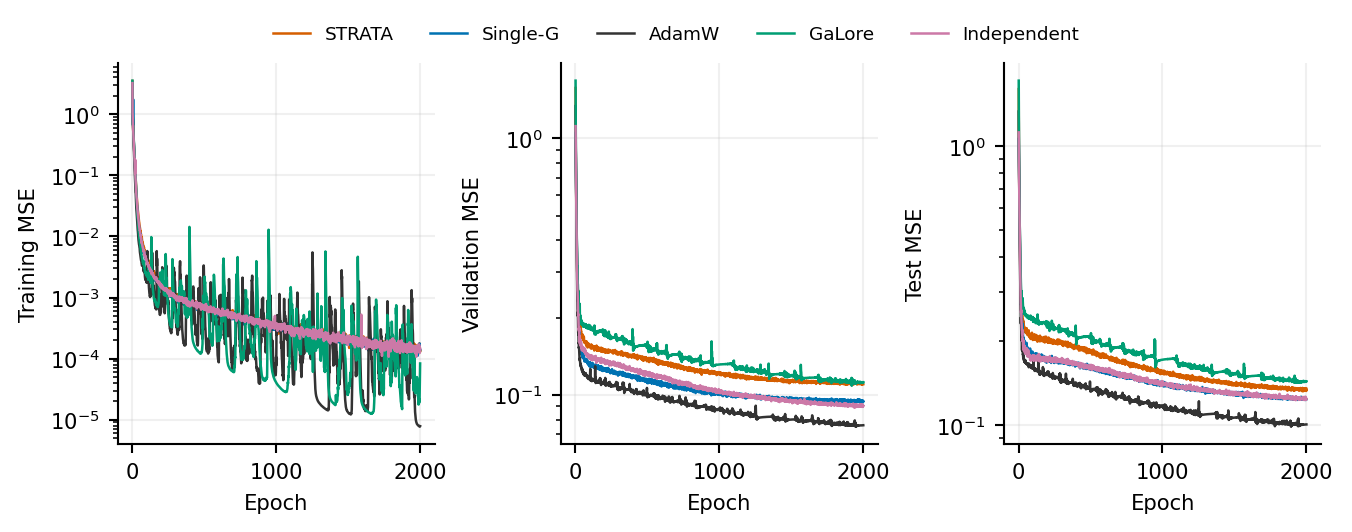
\includegraphics[width=.98\linewidth]{figures/fig_evidence_darcy.png}\caption{Complete 2000-epoch Darcy/FNO loss trajectories: training, validation, and test MSE. Rates are validation-selected from complete two-rate grids; test residual and spectrum never select a curve. All methods and adverse outcomes are retained.}\end{figure}
\paragraph{PubMed mechanism follow-up.} The ten variants and both rates are frozen before follow-up outcomes. Their controls reuse the original two full-method configurations. Freezing after 200 updates also stops variance resets; periodic pooled SVD changes the flag objective. Thus these are explicitly identified interventions, not pure isolated geometry controls.
\begin{table}[htbp]\centering\footnotesize\setlength{\tabcolsep}{3pt}\caption{Complete PubMed/SAGE ablation grid, validation-selected rates, terminal-100 accuracies. Differences are relative to full STRATA. No variant is promoted to the default based on test results.}\label{tab:pubmed-ablations}\begin{adjustbox}{max width=\linewidth}
\begin{tabular}{lrrrr}\toprule Variant & lr & Val & Test & $\Delta$ test (pp)\\\midrule
\rowcolor{oursbg}
full & 1e-03 & 0.71792 & 0.71623 & +0.000 \\
same\_rho & 1e-03 & 0.71302 & 0.70196 & -1.427 \\
reverse\_rho & 3e-04 & 0.69346 & 0.67923 & -3.700 \\
equal\_a & 1e-03 & 0.71646 & 0.71188 & -0.435 \\
no\_residual & 1e-03 & 0.70986 & 0.69363 & -2.260 \\
random\_flag & 1e-03 & 0.69942 & 0.70164 & -1.459 \\
no\_transport & 3e-04 & 0.69988 & 0.67823 & -3.800 \\
frozen\_after\_warmup & 3e-04 & 0.69730 & 0.67639 & -3.984 \\
heterogeneous\_memory & 1e-03 & 0.71310 & 0.70829 & -0.794 \\
periodic\_svd & 1e-03 & 0.70572 & 0.69553 & -2.070 \\
least\_squares\_transport & 1e-03 & 0.70994 & 0.70900 & -0.723 \\
\bottomrule\end{tabular}
\end{adjustbox}\end{table}
\paragraph{Exploratory flag-step sensitivity.} The declared grid is $\xi\in\{10^{-3},10^{-1},10\}$ and $\eta\in\{3\times10^{-4},10^{-3}\}$ for each of STRATA, Single-G and Independent: six equal-budget candidates per method. Defaults remain unchanged. Larger raw-objective steps test whether weak flag motion limits the default protocol. Baseline numerical paths were checked unchanged for all five optimizers over 55 paired updates; all 20 new graph-path smoke tests passed. New runs save float32 bases and evaluate span motion with float64 QR/SVD; old float16 flag snapshots are not used to infer tiny principal angles. The span diagnostic is $D_{\rm span}=\sqrt{1-\lVert Q_{10}^{\top}Q_{1000}\rVert_F^2/r}$, with fresh orthonormal QR factors and represented rank $r$. Independent uses the concatenated subspace union when it has full column rank; excluded rank-deficient matrices are not assigned zero motion.
\begin{table}[htbp]\centering\footnotesize\setlength{\tabcolsep}{3pt}\caption{Matched six-candidate exploratory search per geometric optimizer, selected on validation. Span motion compares the total represented space at checkpoints 10 and 1000, using float64 QR/SVD and averaging eligible matrices. It is not an oracle tracking error.}\label{tab:xi-sweep}\begin{adjustbox}{max width=\linewidth}
\begin{tabular}{lrrrrr}\toprule Method & $\xi$ & lr & Val & Test & Span motion\\\midrule
\rowcolor{oursbg}
STRATA & 10 & 1e-03 & 0.75018 & 0.73383 & 0.129 \\
Single-G & 0.001 & 3e-04 & 0.70666 & 0.67902 & 8.39e-06 \\
Independent & 0.001 & 1e-03 & 0.74190 & 0.74151 & 1.25e-05 \\
\bottomrule\end{tabular}
\end{adjustbox}\end{table}
\begin{table}[htbp]
\centering
\caption{\textbf{Complete flag-step sensitivity profiles.} Each point selects its learning rate on validation after both candidates finish. Test values are reporting only.}
\label{tab:xi-profile}
\begin{adjustbox}{max width=\linewidth}
\begin{tabular}{lrrrr}
\toprule
Method & $\xi$ & lr & Val acc & Test acc \\
\midrule
\rowcolor{oursbg}
STRATA & 0.001 & 1e-03 & 0.71792 & 0.71623 \\
\rowcolor{oursbg}
STRATA & 0.1 & 3e-04 & 0.69918 & 0.67856 \\
\rowcolor{oursbg}
STRATA & 10 & 1e-03 & 0.75018 & 0.73383 \\
Single-G & 0.001 & 3e-04 & 0.70666 & 0.67902 \\
Single-G & 0.1 & 1e-03 & 0.70510 & 0.68944 \\
Single-G & 10 & 3e-04 & 0.69188 & 0.68123 \\
Independent & 0.001 & 1e-03 & 0.74190 & 0.74151 \\
Independent & 0.1 & 1e-03 & 0.72100 & 0.72332 \\
Independent & 10 & 1e-03 & 0.67426 & 0.65143 \\
\bottomrule
\end{tabular}
\end{adjustbox}
\end{table}

\begin{figure}[!htbp]\centering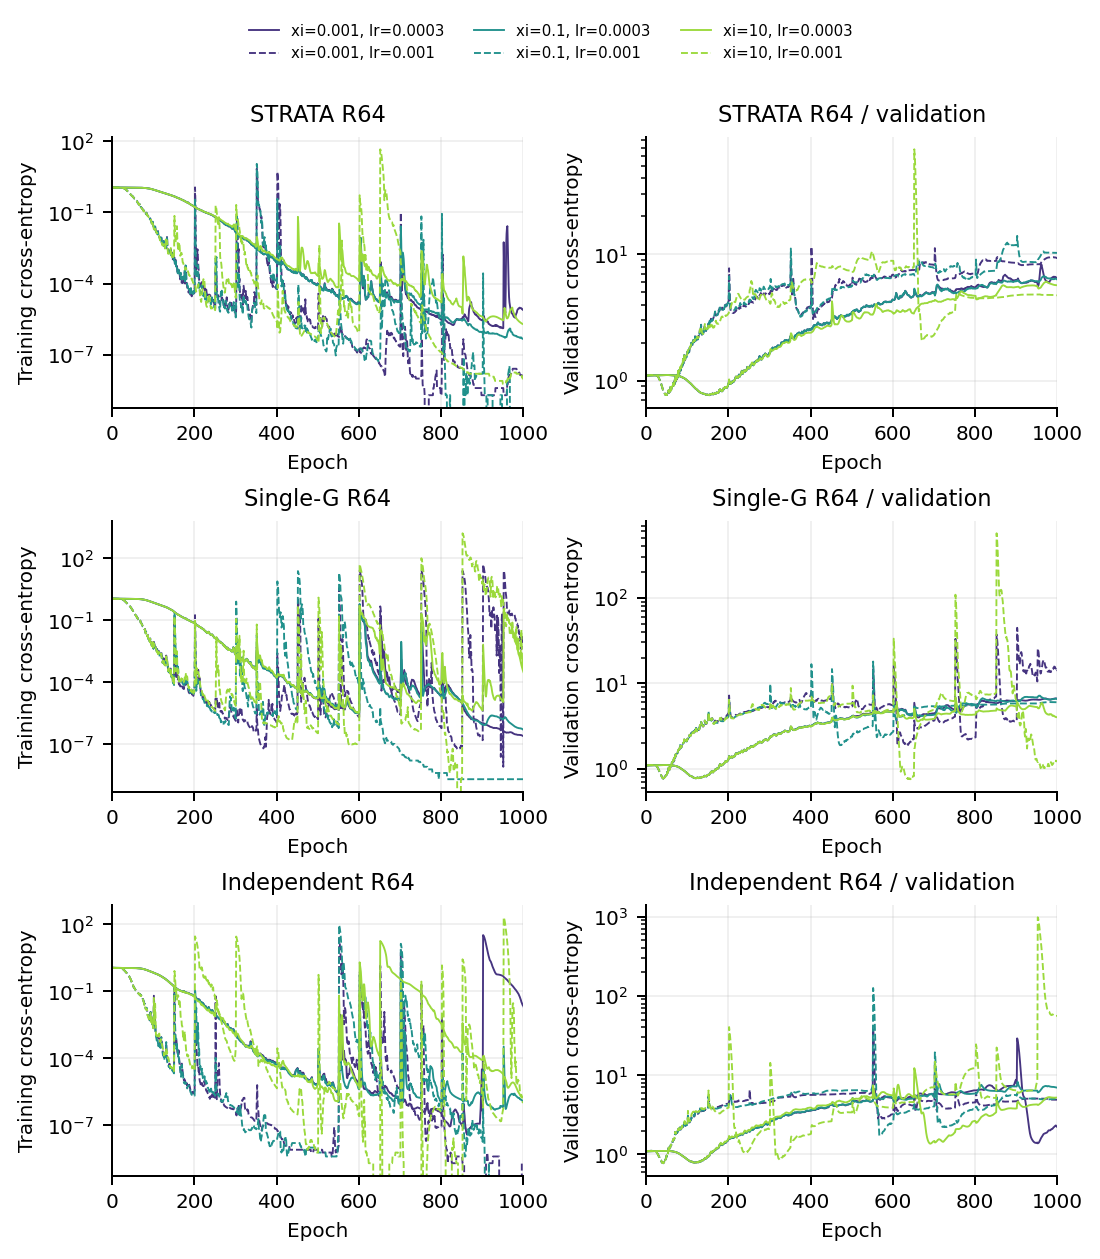
\includegraphics[width=.98\linewidth]{figures/fig_evidence_xi_loss_grid.png}\caption{All 18 completed equal-rank step/rate trajectories, without selection or smoothing. Rows show STRATA, Single-G and Independent; columns show training and validation cross-entropy. Colors denote flag step and line styles distinguish the two learning rates. Every candidate runs 1000 epochs.}\end{figure}
\paragraph{State-matched capacity control.} Same-rank comparisons allocate more optimizer state to STRATA than to Single-Grassmann. We therefore choose the closest integer Single-G rank using initialized tensor storage only, before observing any new accuracy; the target includes probes. Both methods receive the same six-candidate flag-step/rate grid. This is an approximately equal-state comparison, separate from the equal-rank default protocol.
Single-G rank 82 uses 2423128 bytes, versus 2433048 for rank-64 STRATA, a signed difference of -0.408\%. The choice uses exact shape-derived state counts over integer ranks 4--255, including probe-rank saturation, checked against actual initialized storage at four ranks and an archived STRATA final checkpoint; no validation or test score chooses rank.
\begin{table}[htbp]\centering\footnotesize\setlength{\tabcolsep}{3pt}\caption{Completed state-budget control. Rank is fixed from storage alone; every row finishes two rates at each of three flag steps. Default test selects the rate at $\xi=10^{-3}$; six-grid test selects both hyperparameters on validation. Independent uses blocks of dimensions $(16,16,32)$, whose total rank budget is 64. State includes probes and the cached union basis when present.}\label{tab:memory-control}\begin{adjustbox}{max width=\linewidth}
\begin{tabular}{lrrrrr}\toprule Method & State MiB & $\xi_{6}$ & lr$_6$ & Test default & Test six-grid\\\midrule
\rowcolor{oursbg}
STRATA R64 & 2.320 & 10 & 1e-03 & 0.71623 & 0.73383 \\
Single-G R64 & 1.820 & 0.001 & 3e-04 & 0.67902 & 0.67902 \\
Single-G R82 & 2.311 & 0.001 & 1e-03 & 0.72923 & 0.72923 \\
Independent total R64 & 2.195 & 0.001 & 1e-03 & 0.74151 & 0.74151 \\
\bottomrule\end{tabular}
\end{adjustbox}\end{table}
\begin{figure}[!htbp]\centering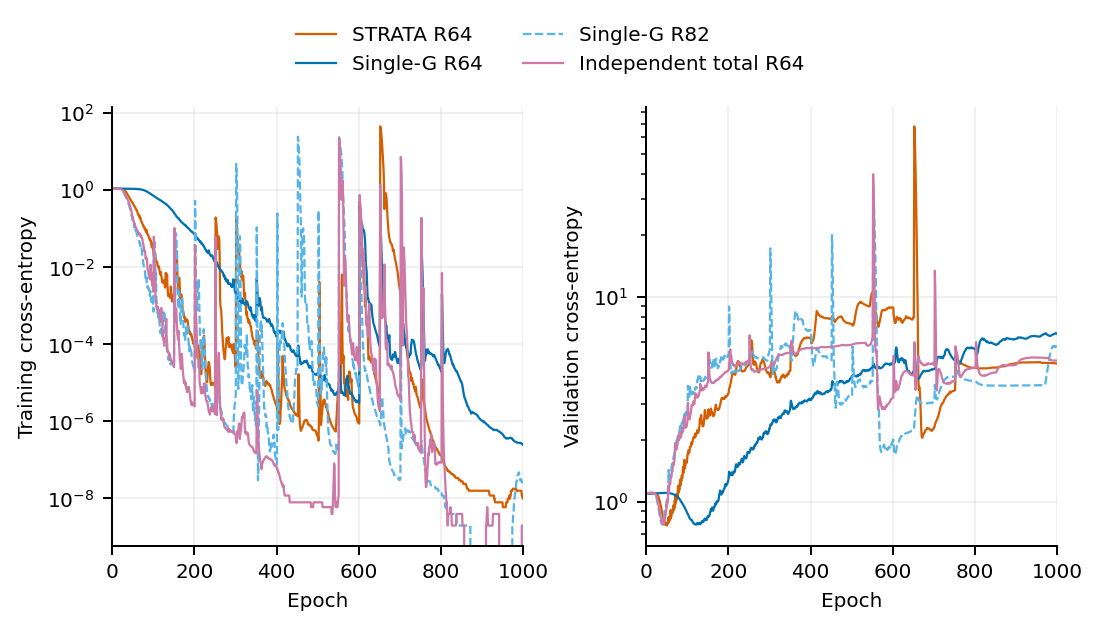
\includegraphics[width=.98\linewidth]{figures/fig_evidence_memory_control.png}\caption{Completed capacity-control training and validation losses after equal six-candidate validation selection. The additional Single-G rank is determined using state storage alone; all six candidates are shown separately below.}\end{figure}
\begin{table}[htbp]\centering\footnotesize\caption{All six completed Single-G state-control candidates. The rank is chosen using storage alone; validation, not test, selects the reported optimum.}\begin{adjustbox}{max width=\linewidth}
\begin{tabular}{rrrr}\toprule $\xi$ & lr & Val acc & Test acc\\\midrule
0.001 & 3e-04 & 0.71554 & 0.71640 \\
0.001 & 1e-03 & 0.73948 & 0.72923 \\
0.1 & 3e-04 & 0.69382 & 0.69613 \\
0.1 & 1e-03 & 0.62916 & 0.61564 \\
10 & 3e-04 & 0.69020 & 0.69950 \\
10 & 1e-03 & 0.72560 & 0.72434 \\
\bottomrule\end{tabular}
\end{adjustbox}\end{table}
\begin{figure}[!htbp]\centering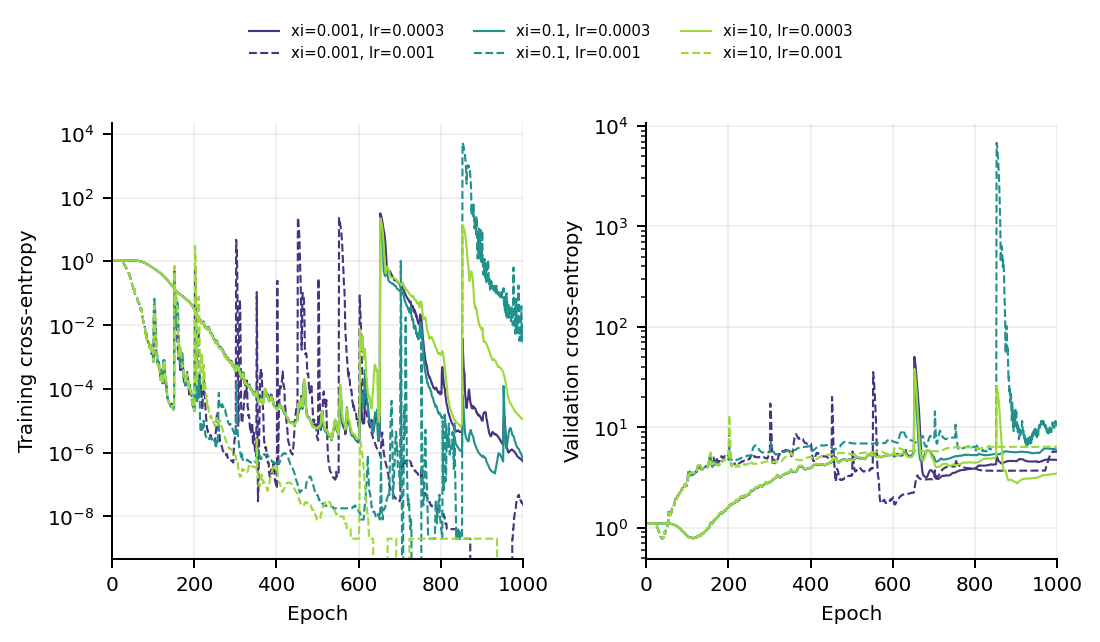
\includegraphics[width=.98\linewidth]{figures/fig_evidence_memory_grid.png}\caption{All six completed Single-G capacity-control training and validation trajectories. No candidate is omitted, selected or smoothed in this grid view.}\end{figure}
